\newpage
\section{Create two functions in R and compute the GMM with the S\&P500 returns}

Adopting the exact same approach as previously, moment conditions are defined as follows:
\begin{equation*}
    Y=    
    \begin{bmatrix}[l]
    E[X^4]-E[X^2]^2(\frac{6}{\nu-4}+3)  \\
    E[X^2]-\frac{\nu}{\nu-2}
    \end{bmatrix}
\end{equation*}

The function will then return the scalar resulting from the quadratic form $Y^TWY$. However, in this particular case we used the S\&P500 sample of returns instead of randomly generated ones; the methodology will be exactly the same: minimizing the moment conditions with respect to $\nu$. The following quadratic form is solved for different parameter candidates and two weight matrices ($W=I$ and $W=\Sigma^{-1}$.
\begin{equation*}
    Y^TWY
\end{equation*}
\begin{equation*}
    W_1=
    \begin{bmatrix}
        1   &0 \\
        0   &1
    \end{bmatrix};\;\;\;\;\;
    W_2=\Sigma^{-1}=
    \begin{bmatrix}[l]
        \frac{1}{\sigma_{m_1,m_1}}    &\frac{1}{\sigma_{m_1,m_2}} \\
        \frac{1}{\sigma_{m_2,m_1}}    &\frac{1}{\sigma_{m_2,m_2}}
    \end{bmatrix}
\end{equation*}

Running the code for the two cases generate a vector containing the output of the minimization problem for every parameter $\nu$ employed. Recall that by the first moment condition $\nu>4$ therefore a parameter list of the following form is set: $\nu_i \in \{5:30\}$. The goal is to find the parameter $\nu$ for which the objective function, i.e. criterion, is minimized, the resulting plots are listed on the following page.
\bigskip\par
The data used in the exercise gives an estimated $\nu$ of:
\begin{equation*}
    \begin{cases}
    \widehat{\nu}_{GMM_{1}}=5 \;\;\text{using W=I}\\
    \widehat{\nu}_{GMM_{2}}=30 \;\;\text{using W=}\Sigma^{-1}
\end{cases}
\end{equation*}

\subsection{W=I}
Why is the convexity apparently disappeared ? The criterion function has a minimum at $\nu_1=5$ and trying to run the code while changing the candidates list to $\nu_i \in \{5:30\}$ won't change the result: the minimum will always be at the first candidate tested. Chapter 2 aims to provide an explanation to this phenomenon.

\subsection{W=$\Sigma^{-1}$}
At first sight it seems correct to have convexity, the problem here is that we have a minimum for the exactly last candidate. Expanding the list of candidates from $\nu_i \in \{5:30\}$ to $\nu_i \in \{5:1000\}$ won't change the outcome, in this case the minimum would be at $\nu=1000$. To understand the phenomenon, the covariance matrix has to be analyzed.
\begin{equation*}
    W=\Sigma=
    \begin{bmatrix}[l]
        31.84035    &8250.907 \\
        8250.90722  &2839215.102
        \end{bmatrix}
\end{equation*}





\newpage

\begin{figure}
    \centering
    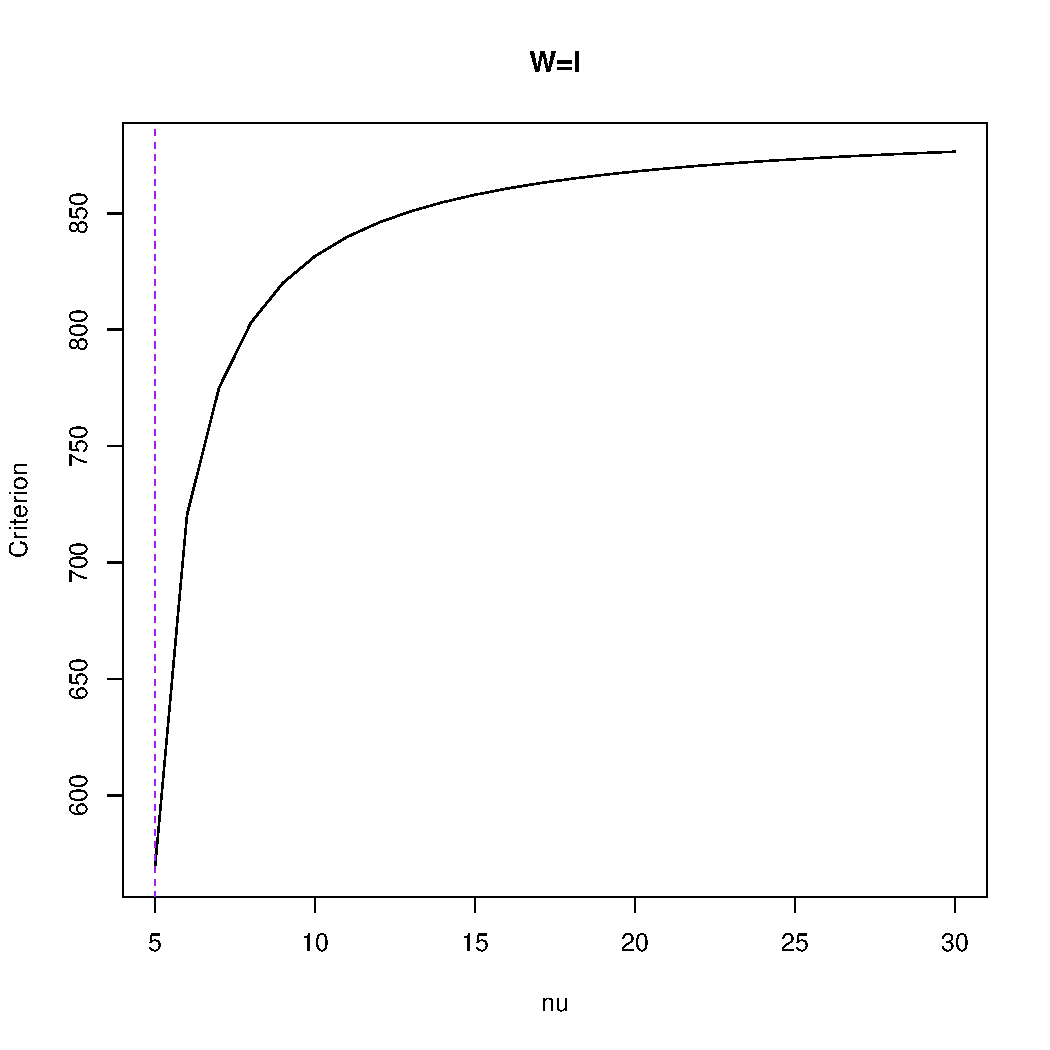
\includegraphics[width=0.7\textwidth]{S&P500_returns_criterion_(W=I).pdf}
    \label{SP500_returns_criterion_I}
    \caption{Output distribution as a function of the candidates $\nu$ using $W=I$}
    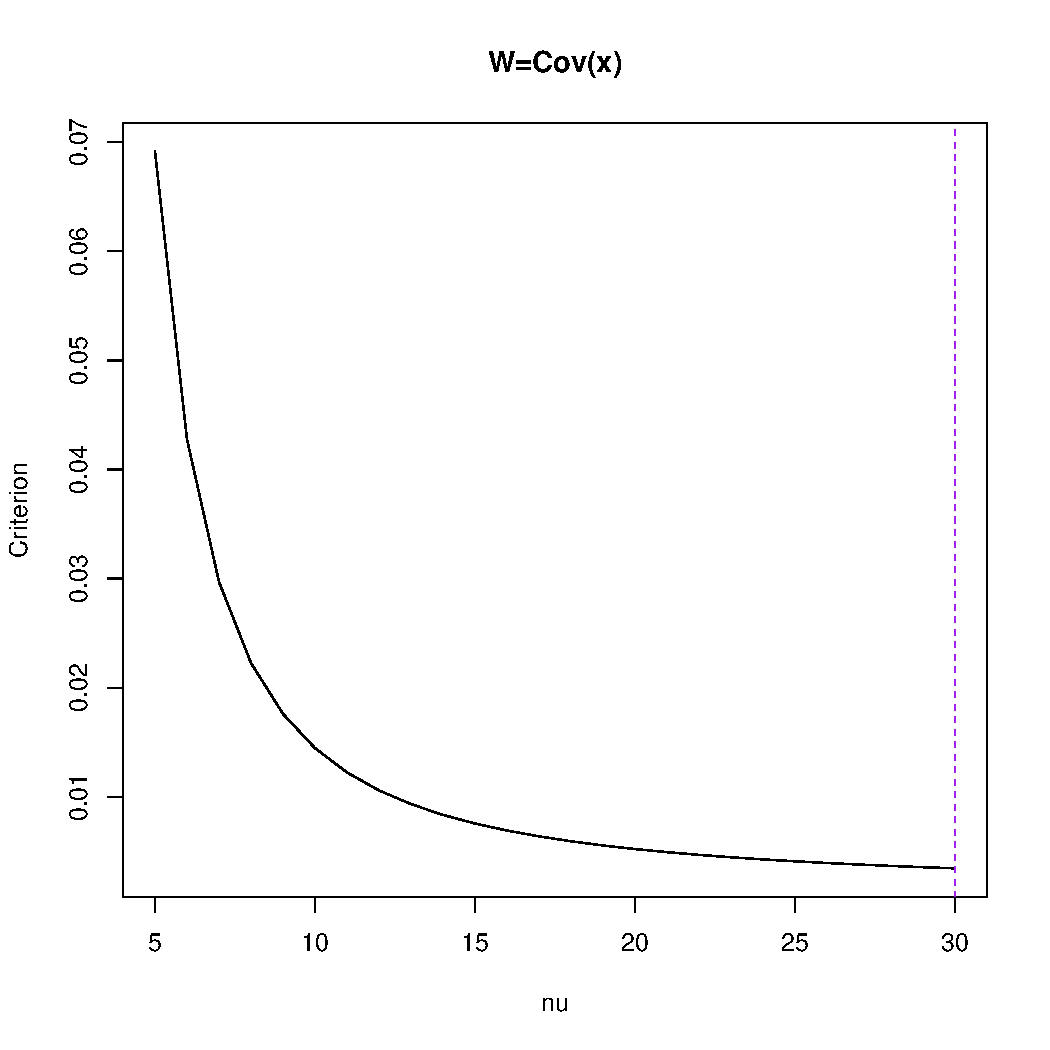
\includegraphics[width=0.7\textwidth]{S&P500_returns_criterion_(W=Sigma^-1).pdf}
    \label{SP500_returns_criterion_W}
    \caption{Output distribution as a function of the candidates $\nu$ using $W=\Sigma^{-1}$}
\end{figure}

\begin{figure}
    \centering
    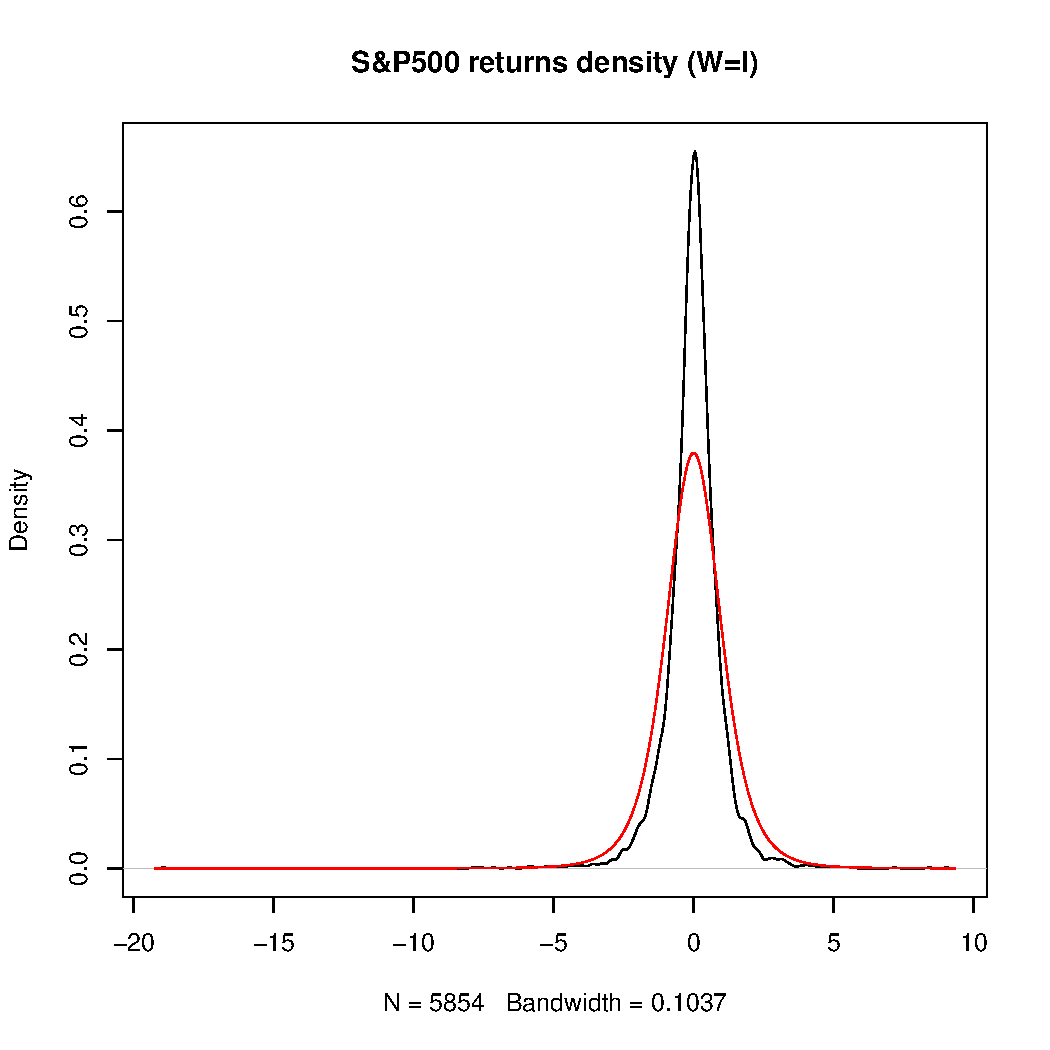
\includegraphics[width=0.7\textwidth]{S&P500_returns_density_(W=I).pdf}
    \label{SP500_returns_density_I}
    \caption{S\&P500 returns density using $W=I$}
    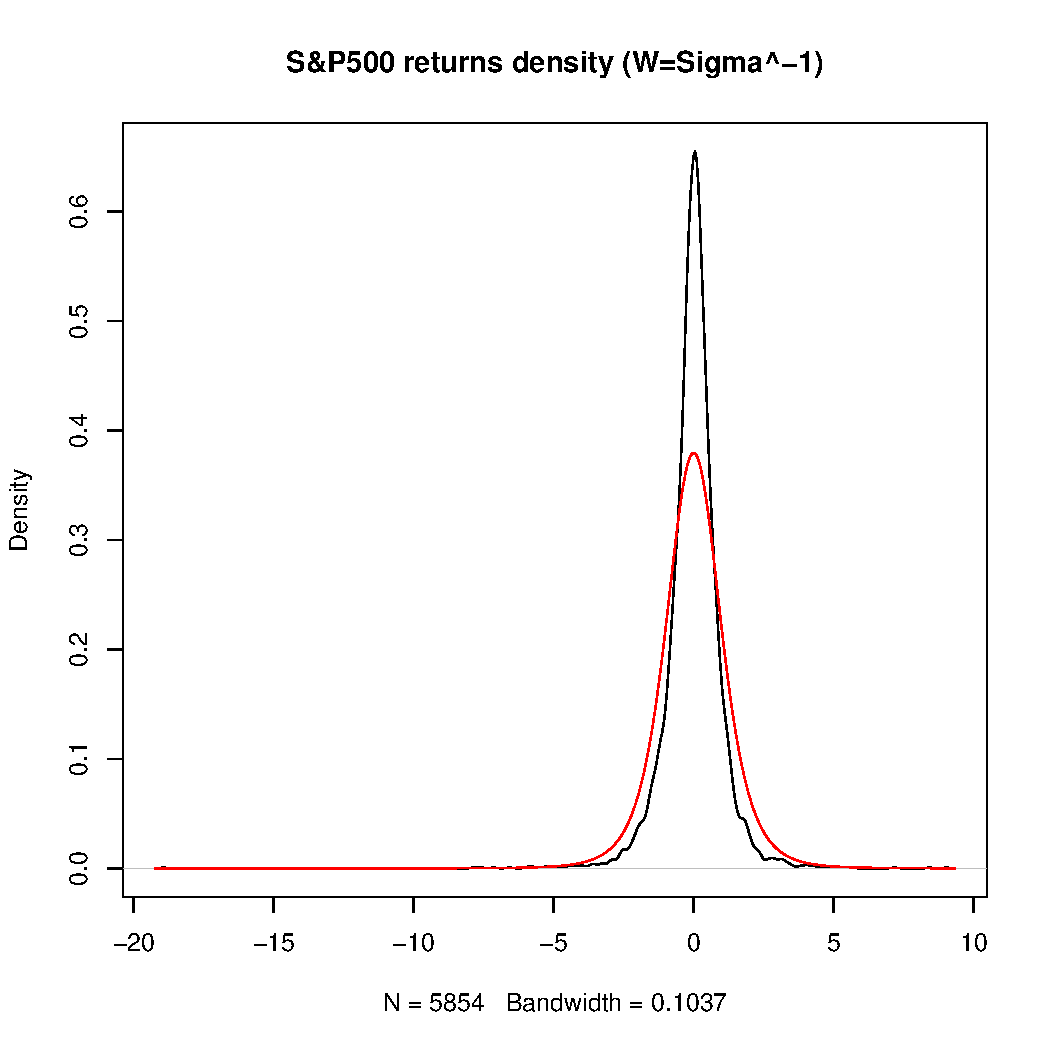
\includegraphics[width=0.7\textwidth]{S&P500_returns_density_(W=Sigma^-1).pdf}
    \label{SP500_returns_density_W}
    \caption{S\&P500 returns density using $W=\Sigma^{-1}$}
\end{figure}